\chapter{Kết quả triển khai và phân tích}
\label{Chapter4}

\section{Mô hình thực nghiệm}
Hệ thống IoT được xây dựng dựa trên kiến trúc IoT bốn lớp được đề xuất. Ở lớp nhận thức, vi điều khiển STM32F411VET6 được sử dụng, hoạt động với tần số 16 MHz. Ở lớp mạng, sử dụng module ESP32 với tần số 240 MHz, đóng vai trò là gateway, tổng hợp và luân chuyển dữ liệu lên máy chủ với cấu hình của máy chủ được trình bày trong bảng \ref{tab:server-config}. Đối với quá trình trao đổi khóa giữa máy chủ và gateway, mô hình được cấu hình sẵn thời gian giữa các lần trao đổi khóa là một phút, nhằm dễ đánh giá việc chi phí tính toán của thuật toán ECDH ảnh hưởng đến hệ thống như thế nào. Tuy nhiên, thời gian trao đổi khóa có thể được cấu hình khác nhau trong thực tế, tùy vào khả năng tính toán của hệ thống, năng lượng tiêu thụ và yêu cầu về bảo mật. Thời gian giữa mỗi lần truyền dữ liệu được đặt là 1 ms.

\begin{table}[ht]
\centering
\small
\caption{Cấu hình máy chủ}
\label{tab:server-config}
\renewcommand{\arraystretch}{1.2} % Increase vertical spacing
\begin{tabular}{|p{3cm}|p{10cm}|}
\hline
\textbf{Thành phần} & \textbf{Cấu hình} \\
\hline
OS      & Ubuntu 18.04.6 LTS \\
RAM     & 7.8 GiB \\
Storage & 97 GiB \\
CPU     & Intel(R) Xeon(R) CPU E5504 2.00 GHz \\
\hline
\end{tabular}
\end{table}

\section{Kết quả, phân tích và đánh giá}
Phần này nêu ra các kết quả thực hiện và hiệu suất của hệ thống. Đồng thời, đánh giá một số ưu nhược điểm của hệ thống cũng như khả năng chống lại một số cuộc tấn công phổ biến.
\subsection{Kết quả thực hiện}
Trên MCU STM32F411VET6, các kỹ thuật bao gồm kiến trúc khung truyền, kỹ thuật tạo khóa phiên và mã hóa dữ liệu sử dụng thuật toán mã hóa nhẹ Ascon-128a đã được triển khai thành công. Hình \ref{fig:stm32log} trình bày kết quả thực hiện mã hóa và tạo khóa phiên bằng Debugger trên công cụ CubeIDE. Đối với mỗi quá trình tạo khóa và mã hóa thành công, các biến kiểm tra sẽ được đặt thành 1 để báo quá trình thành công. Giá trị \textit{session\_key\_index} thể hiện thứ tự phiên hiện tại trong quá trình giao tiếp, là tham số được sử dụng trong hàm tạo khóa phiên.
\begin{figure}[h]
    \centering
    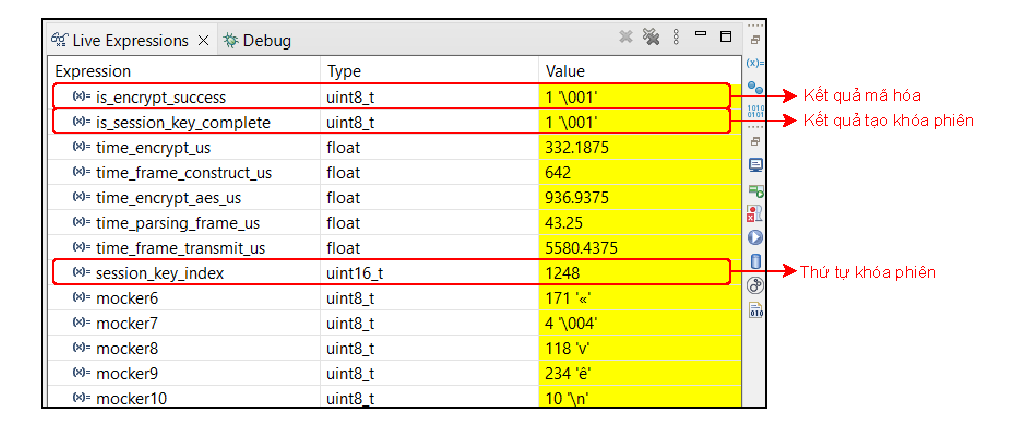
\includegraphics[width=0.9\linewidth]{stm32log.pdf}
    \caption{Kết quả thực hiện trên MCU STM32F411VET6}
    \label{fig:stm32log}
\end{figure}

Khi hệ thống được reboot, quá trình khởi tạo ngay lập tức hoạt động. ESP32 gửi một tín hiệu yêu cầu gói tin khởi tạo từ máy chủ. Sau đó, máy chủ sẽ xác minh thiết bị yêu cầu và gửi về dữ liệu khởi tạo. Dữ liệu khởi tạo này sau đó sẽ được ESP32 tiếp tục chuyển tiếp xuống STM32 ở lớp nhận thức. Kết quả thực hiện quá trình này được trình bày trong hình \ref{fig:initlog}.

\begin{figure}[h]
    \centering
    \hspace*{-0.7cm}
    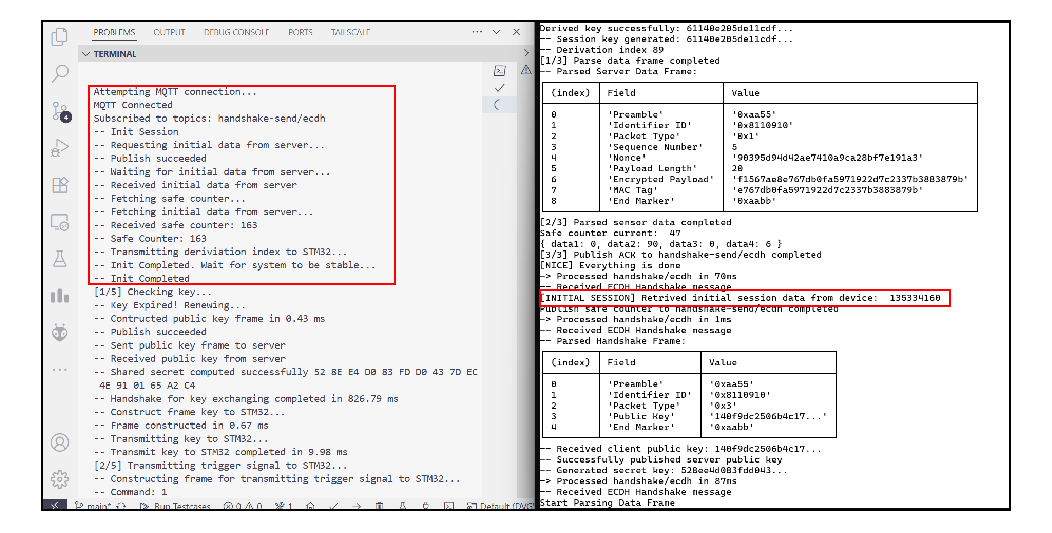
\includegraphics[width=1.08\linewidth]{initlog.pdf}
    \caption{Quá trình khởi tạo khi reboot}
    \label{fig:initlog}
\end{figure}

Kỹ thuật trao đổi khóa sử dụng thuật toán ECDH được triển khai thành công trên ESP32 IoT Gateway và hệ thống Backend. Thứ tự thực hiện quá trình trao đổi khóa được thực hiện chính xác bao gồm gửi khóa chung, nhận khóa chung và tính toán khóa bí mật. Các khóa chung khi publish đều được cấu trúc bằng khung truyền. Hình \ref{fig:logecdh} trình bày kết quả thực hiện trên ESP32 Gateway và máy chủ.

\begin{figure}[h]
    \centering
    \hspace*{-0.7cm}
    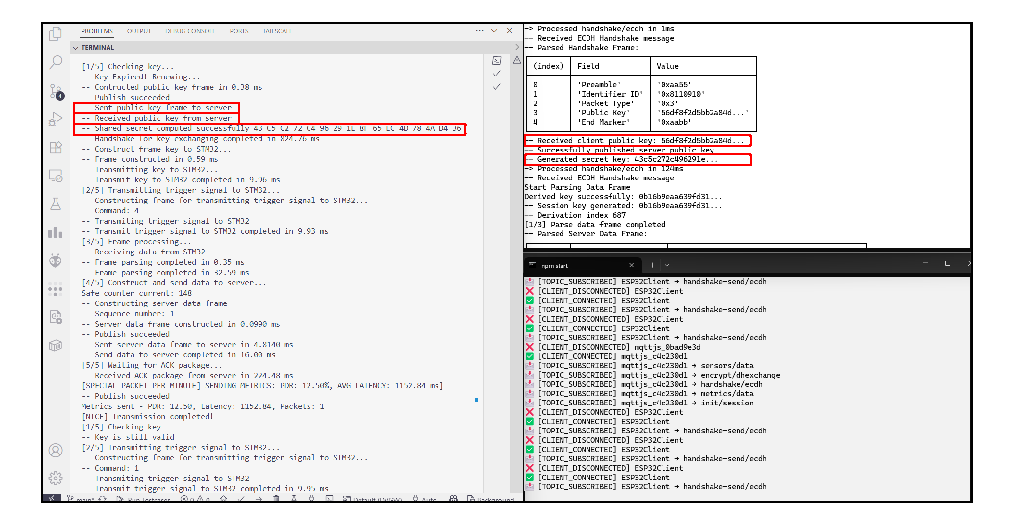
\includegraphics[width=1.08\linewidth]{ecdhlog.pdf}
    \caption{Quá trình trao đổi khóa giữa gateway và máy chủ}
    \label{fig:logecdh}
\end{figure}

Quá trình truyền dữ liệu được triển khai thành công theo đúng trình tự được trình bày trong hình \ref{fig:system} và \ref{fig:trans-sys}. Trên ESP32, quá trình truyền được chia thành năm giai đoạn chính: (1) kiểm tra khóa hiện tại, (2) gửi tín hiệu kích hoạt đến vi điều khiển STM32 tại lớp nhận thức, (3) nhận và phân giải khung dữ liệu từ STM32, (4) tạo khung truyền dữ liệu mới để gửi lên máy chủ, và (5) chờ nhận tín hiệu xác nhận (ACK) từ máy chủ. 
Ở phía máy chủ, sau khi tiếp nhận khung truyền, dữ liệu sẽ được giải mã và xác thực. Nếu dữ liệu hợp lệ, máy chủ sẽ phản hồi tín hiệu ACK để xác nhận thành công và kết thúc phiên truyền. Các kết quả giao tiếp trên được trình bày trong hình \ref{fig:datalog}.
\begin{figure}[h]
    \centering
    \hspace*{-0.7cm}
    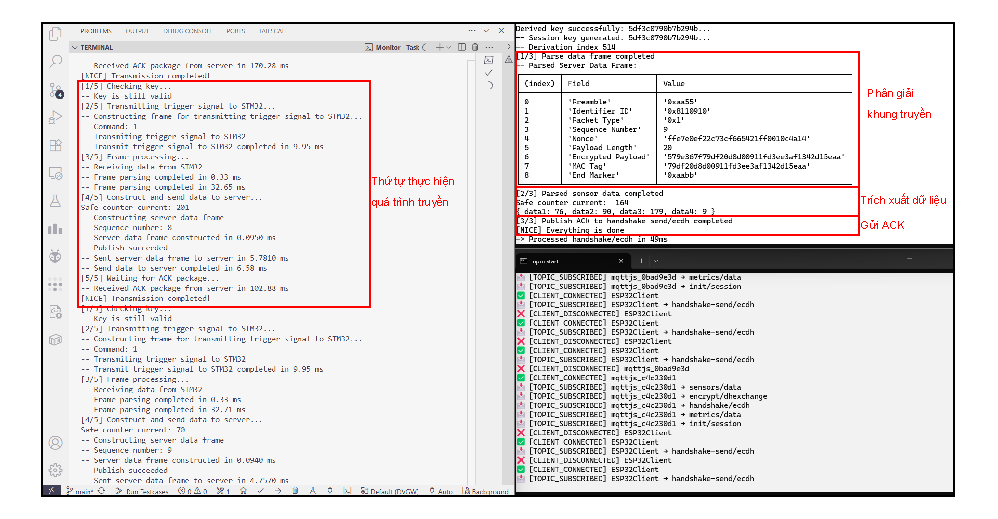
\includegraphics[width=1.08\linewidth]{datalog.pdf}
    \caption{Quá trình truyền dữ liệu}
    \label{fig:datalog}
\end{figure}

Cơ chế \textit{Safe counter} cũng được triển khai thành công trên cả ESP32 IoT Gateway và máy chủ. Khi phát hiện có dấu hiệu của brute-force thông qua việc máy chủ từ chối quá nhiều gói tin trong khoảng thời gian ngắn, máy chủ sẽ gửi một yêu cầu tạo lại \textit{sequence number} mới thông qua\textit{safe counter}. Hình \ref{fig:sclog} trình bày quá trình cập nhật và đồng bộ \textit{sequence number} mới giữa gateway và máy chủ.

\begin{figure}[h]
    \centering
    \hspace*{-0.7cm}
    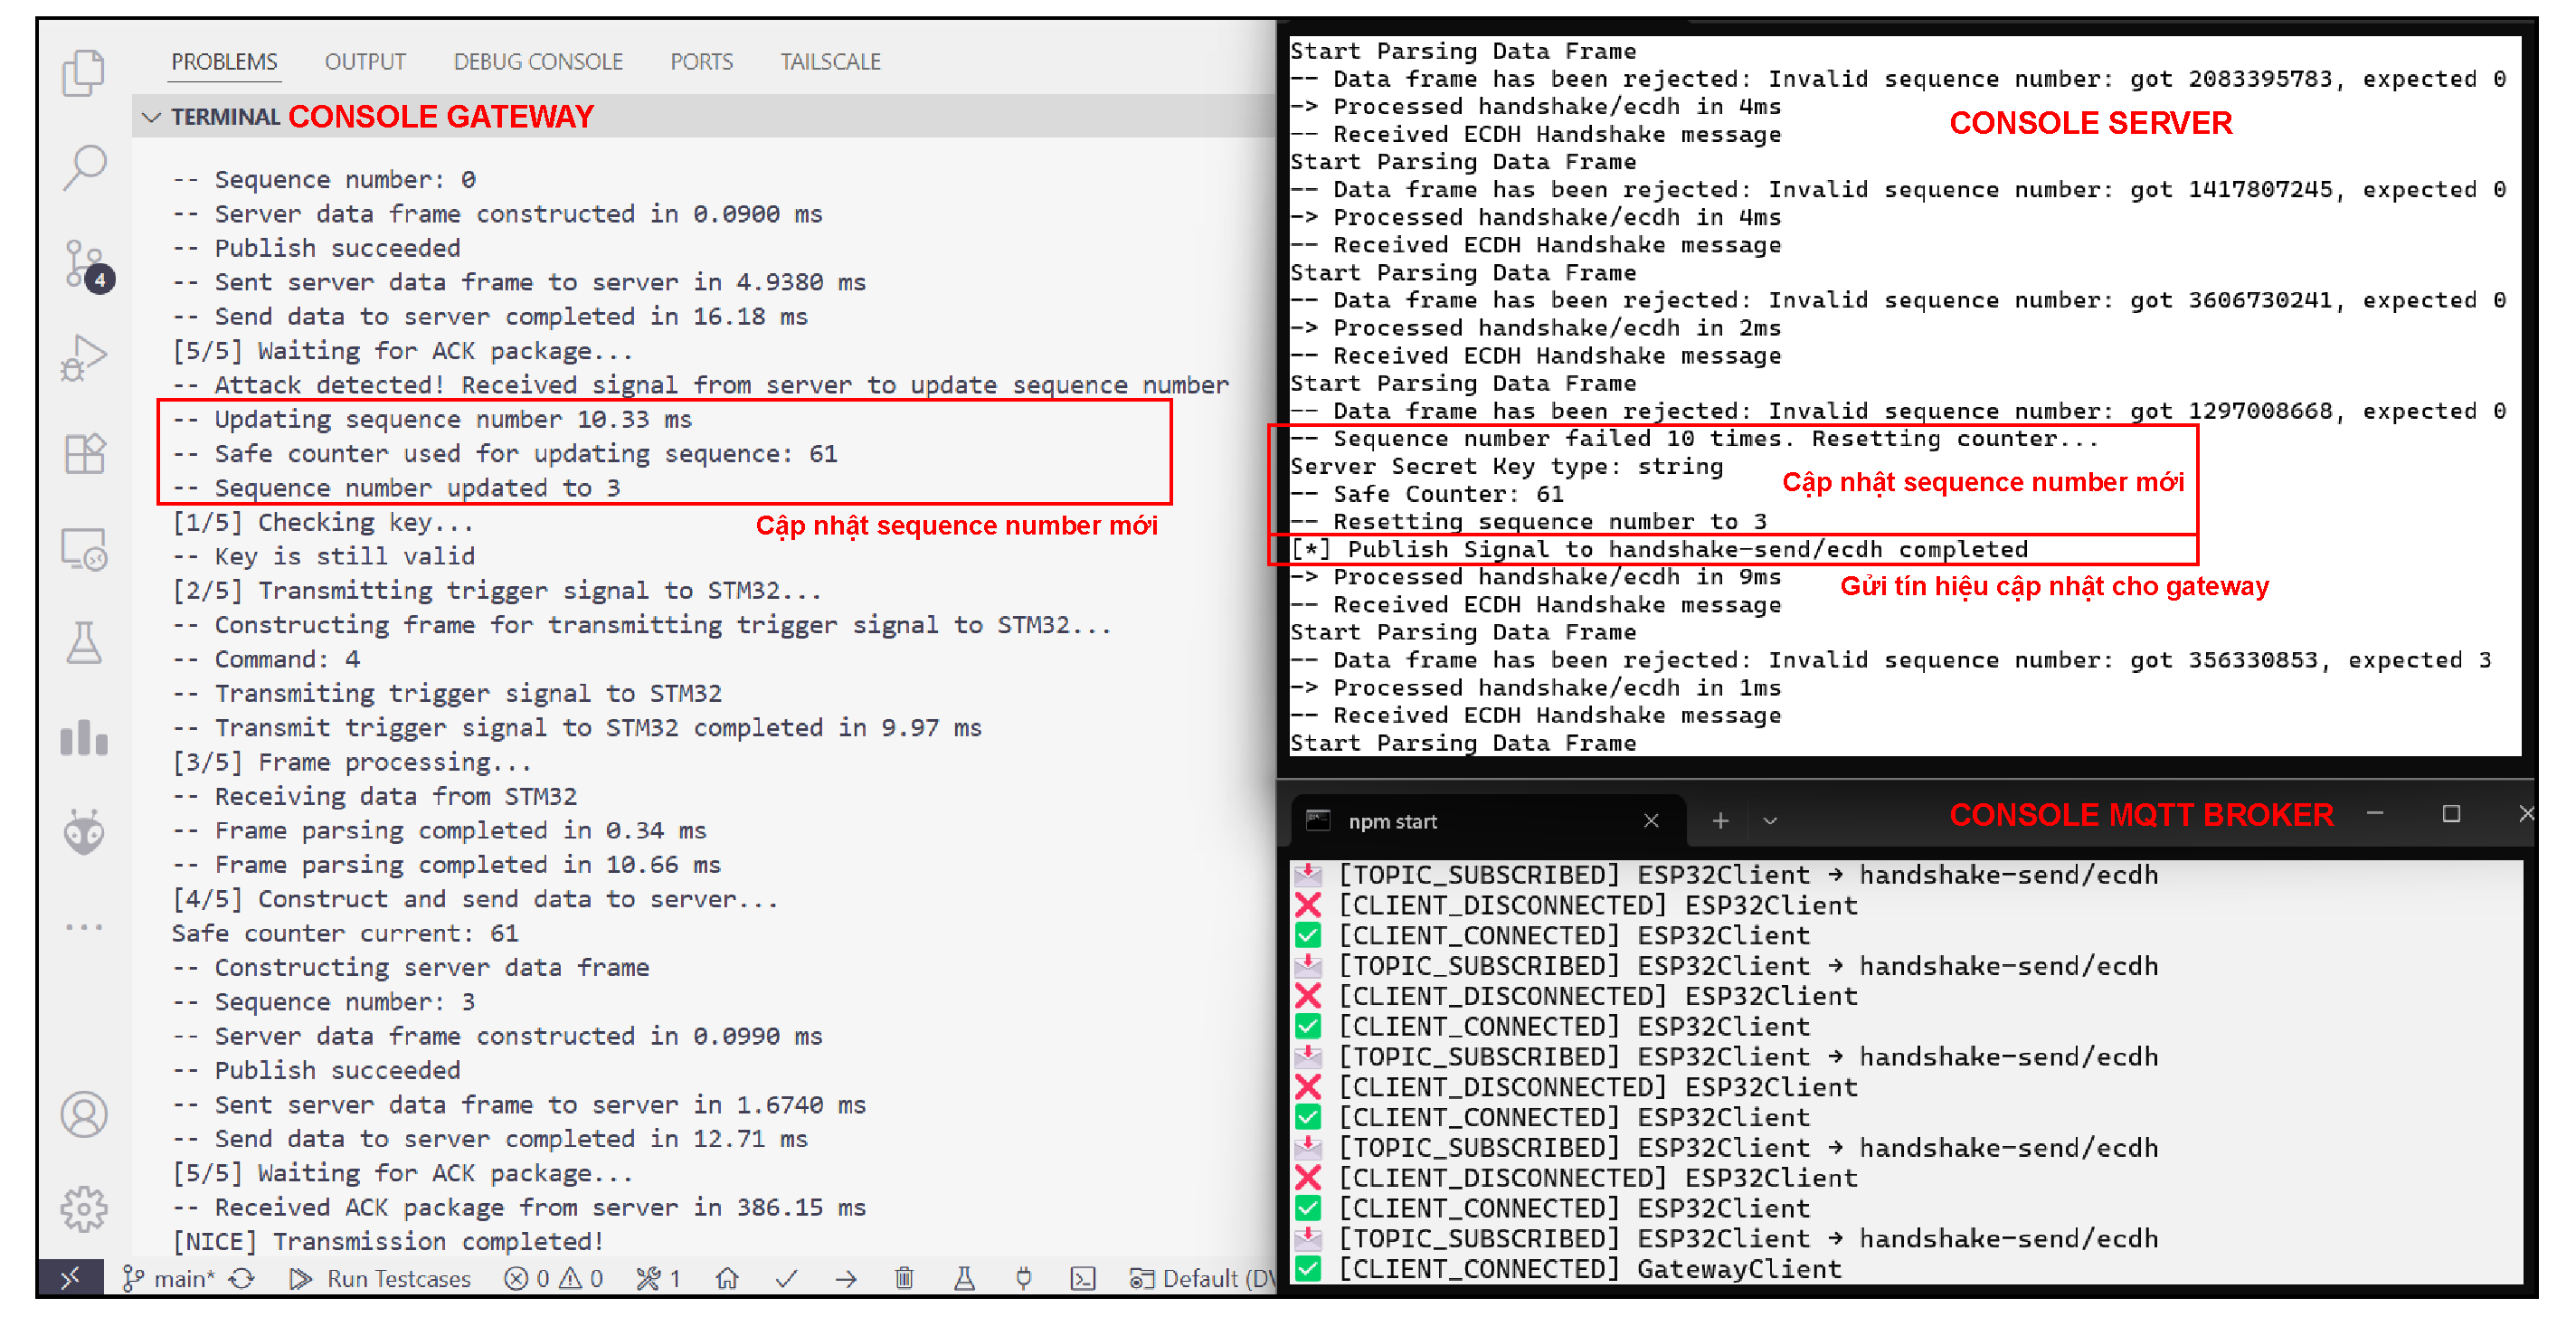
\includegraphics[width=1.08\linewidth]{sclog.pdf}
    \caption{Quá trình thực hiện cơ chế \textit{safe counter}}
    \label{fig:sclog}
\end{figure}

\subsection{Đánh giá}
\label{sec:res}
Hệ thống được đánh giá dựa trên quá trình trao đổi dữ liệu liên tục trong 120 phút, với các kết quả được trình bày trong hình \ref{fig:ke}, \ref{fig:esp32} và hình \ref{fig:stm32}. Kết quả này tập trung vào hiệu suất của hai thiết bị công suất thấp ở lớp nhận thức và lớp mạng. Đầu tiên là đánh giá với STM32F411VET6 ở lớp nhận thức. STM32 thực hiện việc cấu hình khung truyền PG1 với thời gian trung bình là 0.634 ms. Truyền khung PG1 bằng UART lên gateway có thời gian trung bình là 5.58 ms. Thuật toán Ascon-128a có thời gian mã hóa trung bình là 0.328 ms, cho thấy hiệu năng vượt trội so với thuật toán AES, vốn được triển khai tương tự bằng thư viện X-CUBE-CRYPTOLIB và có thời gian mã hóa trung bình là 0.936 ms trên lõi ARM Cortex-M4. Quá trình phân giải khung truyền GP1 từ gateway có thời gian trung bình là 0.374 ms; khung truyền GP2 có thời gian trung bình là 0.023 ms. Sự khác biệt lớn về thời gian trong quá trình phân giải phần lớn là do việc giải mã khóa và tính toán thẻ xác thực ở khung truyền GP1.

Ở lớp mạng, ESP32 thực hiện việc phân giải PG1 từ STM32 trong thời gian trung bình 0.35 ms. Cấu hình khung truyền GP1 có thời gian trung bình là 0.57 ms, trong khi đó thời gian cấu hình GP2 có thời gian trung bình là 0.014 ms. Thời gian truyền khung truyền GP2 dùng UART xuống lớp nhận thức có thời gian trung bình là 9.01 ms. Quá trình trao đổi khóa bao gồm việc tạo cặp khóa cá nhân (private key)/khóa công khai (public key) và tính toán khóa bí mật có thời gian trung bình lần lượt là 335.08 ms và 335.46 ms. Tuy nhiên, việc trao đổi khóa chỉ được thực hiện sau một khoảng thời gian cố định, vì vậy nếu xét về tổng thể sẽ không ảnh hưởng nhiều đến toàn bộ hiệu suất của hệ thống. Thời gian trung bình cấu hình khung truyền GS1 và GS2 lần lượt là 0.28 ms và 0.033 ms. Mặc dù GS2 có nhiều trường cần cấu hình hơn GS1, nhưng GS2 chỉ thực hiện việc tách trường dữ liệu và thẻ xác thực từ khung PG1 mà không thực hiện tính toán nào thêm. Vì thế, việc cấu hình GS2 nhanh hơn nhiều so với GS1, khi mà GS1 cần phải tính toán thẻ xác thực trong quá trình cấu hình. Thời gian tính toán khóa phiên ở mỗi phiên truyền dữ liệu có thời gian trung bình là 1.189 ms.

Lệnh ACK phản hồi từ máy chủ, báo hiệu phiên truyền thành công, có độ trễ trung bình là 29.58 ms, tính từ lúc khung truyền GS tới máy chủ và gateway nhận được ACK. Tuy nhiên, độ trễ này là không cố định do phụ thuộc phần lớn vào tốc độ mạng cũng như hiệu suất của máy chủ; vì vậy, nếu triển khai ở một số hệ thống khác thì độ trễ sẽ có thể khác. Tổng thời gian truyền được tính từ lúc STM32 nhận được tín hiệu kích hoạt từ gateway cho đến khi gateway nhận được ACK là 51.09 ms.

\begin{figure}[h]
    \centering
    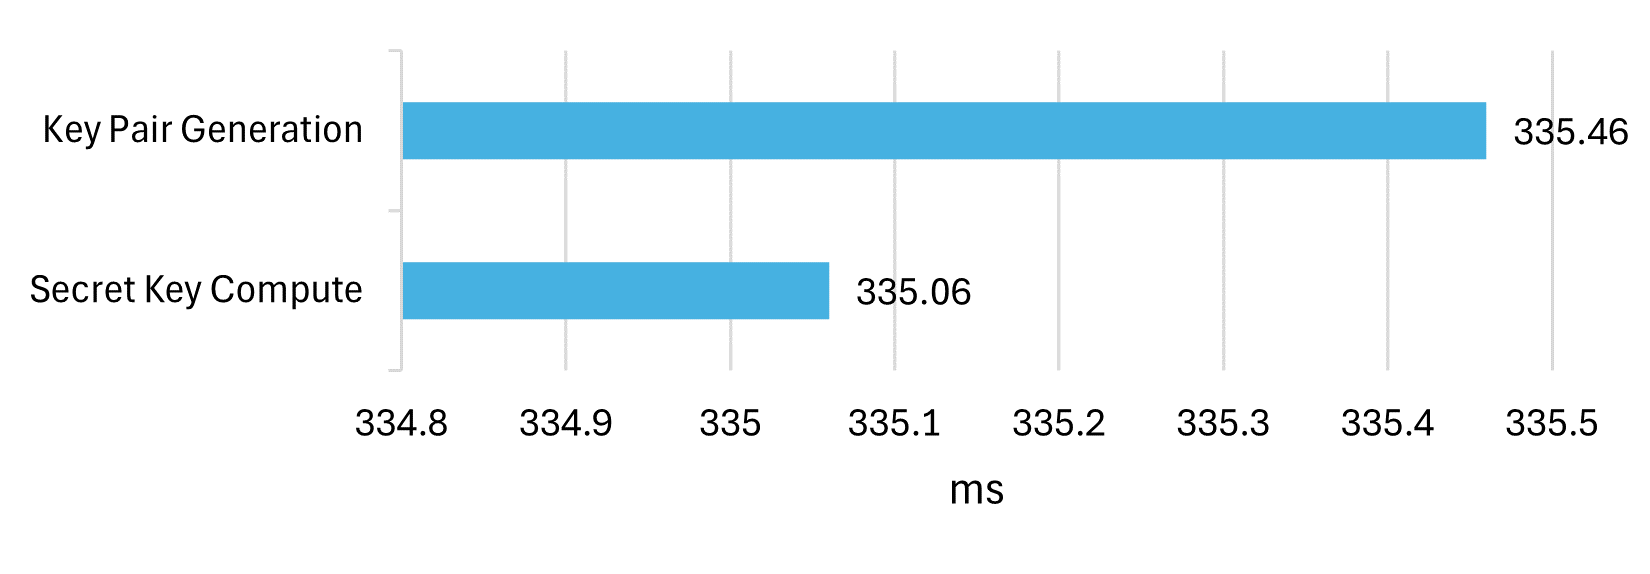
\includegraphics[width=0.8\linewidth]{ke.png}
    \caption{Thời gian thực thi quá trình trao đổi khóa trên ESP32}
    \label{fig:ke}
\end{figure}

\begin{figure}[h]
    \centering
    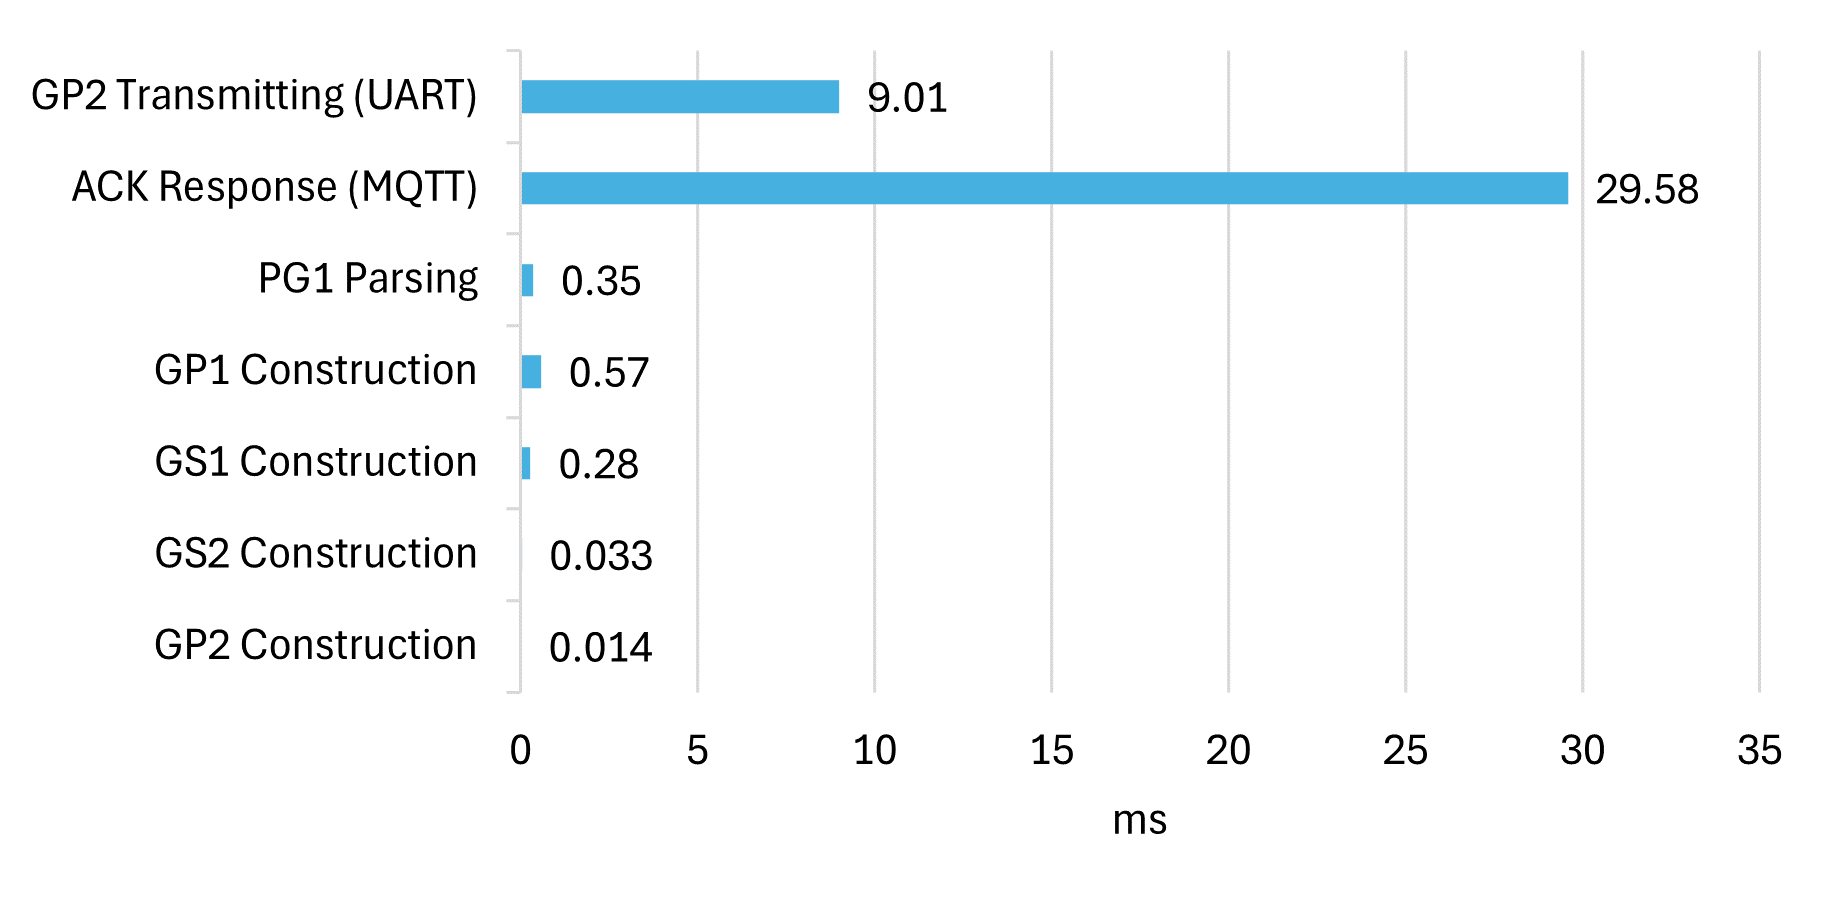
\includegraphics[width=0.8\linewidth]{esp32.png}
    \caption{Đánh giá hiệu suất thực thi các tác vụ của ESP32}
    \label{fig:esp32}
\end{figure}

\begin{figure}[h]
    \centering
    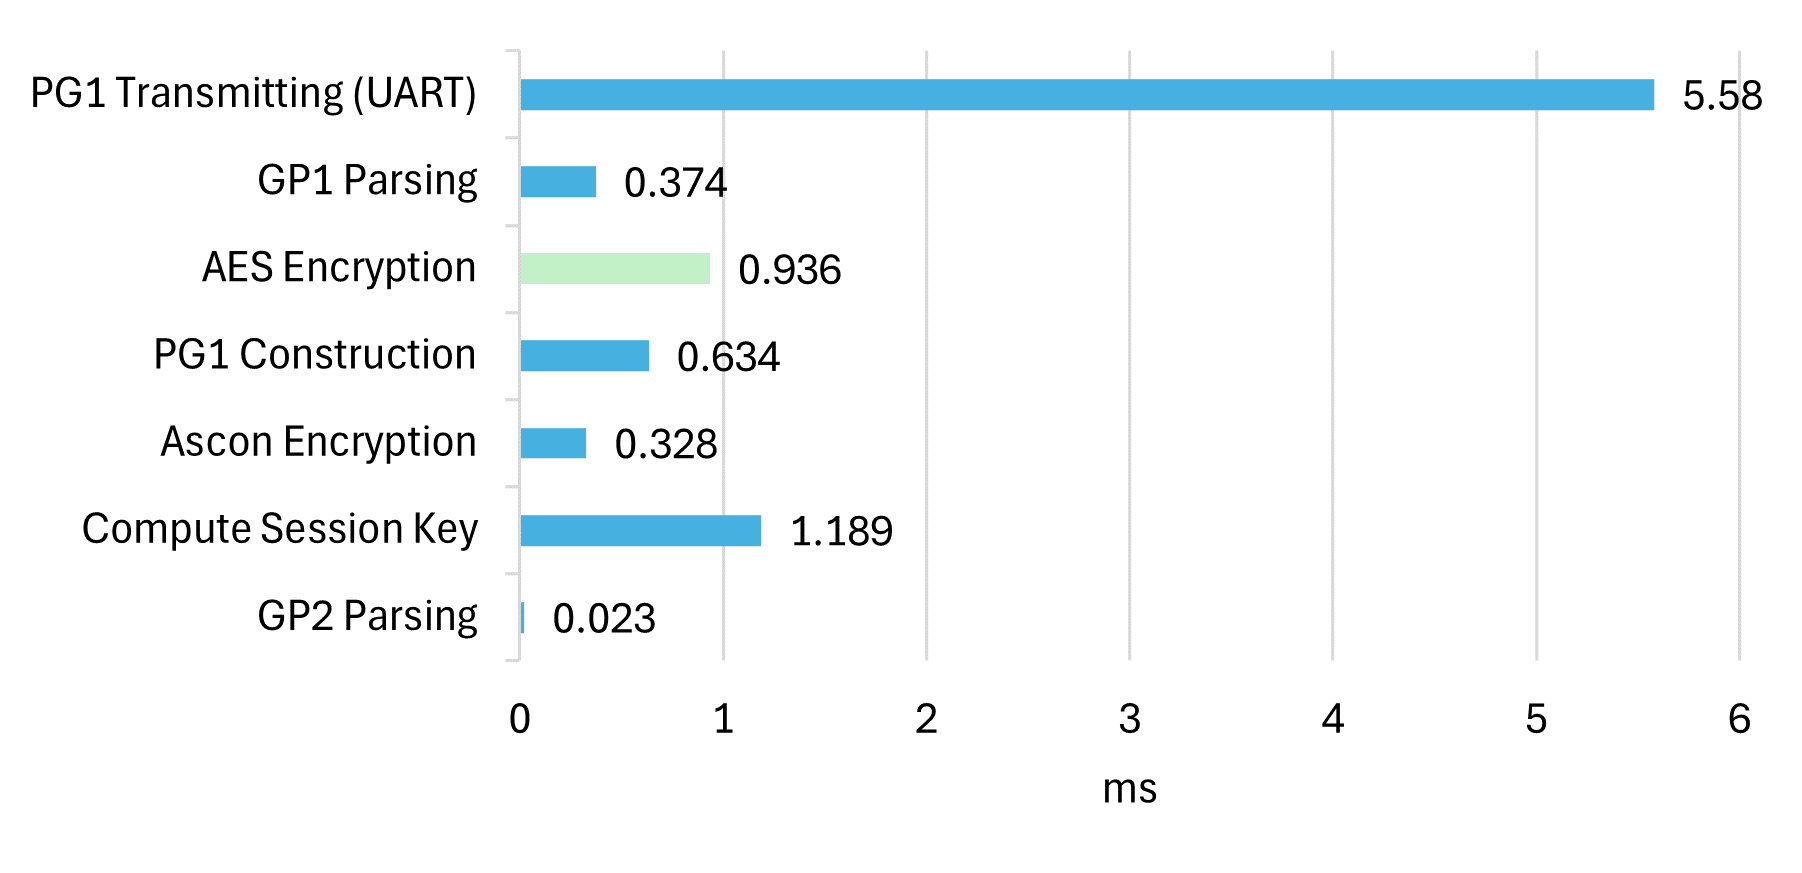
\includegraphics[width=0.8\linewidth]{stm32-2.png}
    \caption{Đánh giá hiệu suất thực thi các tác vụ của STM32F411VET6}
    \label{fig:stm32}
\end{figure}

Trong khoảng thời gian 120 phút thực nghiệm, gateway đã thực hiện truyền tổng cộng 147,682 gói tin. Một gói tin truyền thành công được định nghĩa là gói tin được mã hóa đúng cách và máy chủ có thể giải mã đúng gói tin đó. Tỷ lệ truyền gói tin thành công (Packet Delivery Ratio - PDR) là một thông số quan trọng trong việc đánh giá mức độ toàn vẹn của hệ thống được tính toán sau mỗi phút truyền dữ liệu, được tính toán với công thức sau:
\[
\text{PDR} = \frac{N_{\text{successful}}}{N_{\text{total}}} \times 100\% 
\]

\begin{align*}
\text{Trong đó:} \quad & N_{\text{successful}} \text{ là số gói tin được nhận thành công tại đích (gói/phút),} \\
                       & N_{\text{total}} \text{ là tổng số gói tin được gửi từ nguồn (gói/phút).}
\end{align*}

Biểu đồ trong Hình \ref{fig:packet} minh họa số lượng gói tin được truyền trong mỗi phút trong suốt 120 phút hoạt động liên tục, với số lượng trung bình đạt 1231 gói/phút. Biểu đồ trong hình \ref{fig:pdr} cho thấy tỷ lệ truyền gói tin mỗi phút cũng trong tổng thời gian 120 phút. Kết quả cho thấy tỷ lệ 100\% được duy trì trong phần lớn thời gian truyền, trong các khoảng thời gian còn lại, tỷ lệ được duy trì ổn định trong khoảng từ 99.8\% cho đến 99.975\%. Tỷ lệ truyền gói tin trung bình là 99.99\%, cho thấy mức độ ổn định và toàn vẹn của hệ thống trong suốt quá trình thực nghiệm. Bảng \ref{tab:performance_metrics} tóm tắt các chỉ số hiệu năng, bao gồm tỷ lệ truyền thành công trung bình, số gói tin trên mỗi khoảng thời gian, và thời gian truyền cho mỗi gói tin.

\begin{figure}[H]
    \centering
    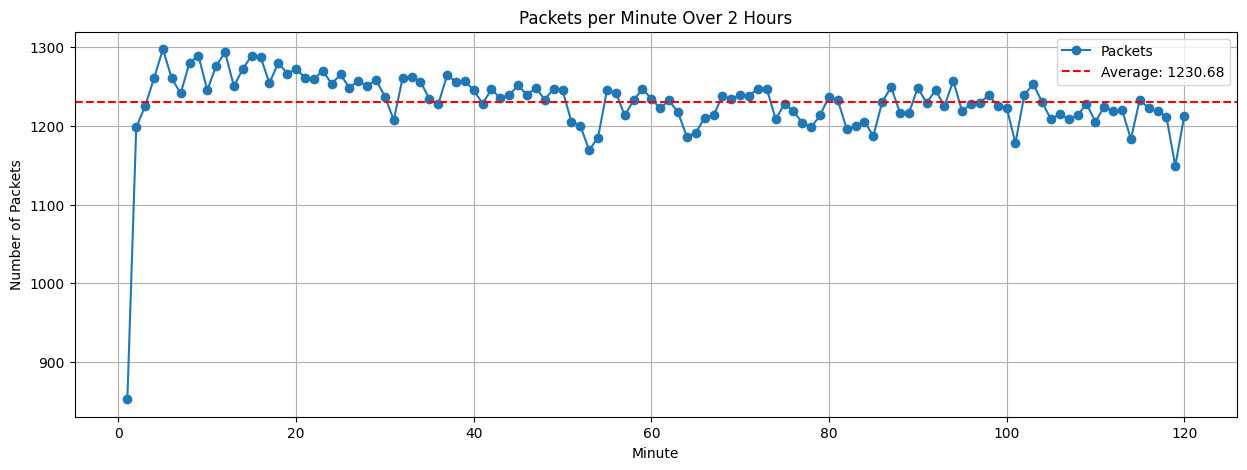
\includegraphics[width=0.9\linewidth]{packet.png}
    \caption{Số lượng gói tin truyền mỗi phút}
    \label{fig:packet}
\end{figure}

\begin{figure}[H]
    \centering
    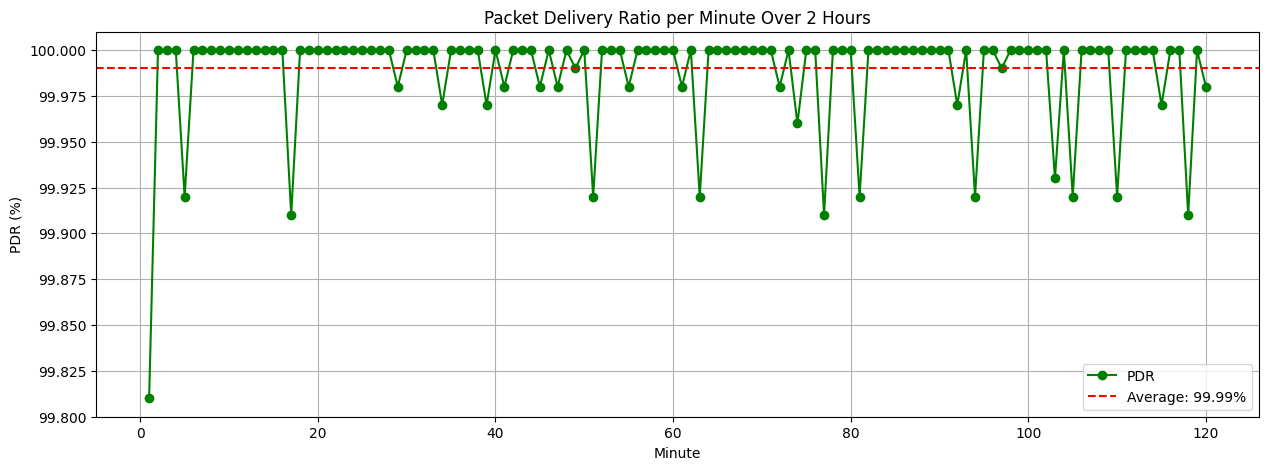
\includegraphics[width=0.9\linewidth]{pdr.png}
    \caption{Tỷ lệ truyền gói tin mỗi phút}
    \label{fig:pdr}
\end{figure}

\begin{table}[H]
    \centering
    \small
    \caption{Bảng đánh giá hiệu năng trong 120 phút}
    \label{tab:performance_metrics}
    \begin{tabular}{|p{10cm}|p{4cm}|}
        \hline
        \textbf{Thông số} & \textbf{Giá trị} \\
        \hline
        Tổng số gói tin truyền & 147,682 gói tin \\
        Thời gian truyền trung bình & 51.09 ms \\
        Số gói tin truyền trung bình mỗi phút & 1231 gói tin \\
        Tỷ lệ truyền thành công (PDR) & 99.99\% \\
        \hline
    \end{tabular}
\end{table}

Dung lượng bộ nhớ của hệ thống IoT trên ESP32 và STM32 được cung cấp bởi công cụ lập trình PlatformIO và Cube IDE, hiển thị tổng số byte RAM và FLASH được sử dụng trong quá trình nạp firmware. Chi tiết trình bày trong bảng \ref{tab:memory}.

\begin{table}[h]
\centering
\small
\caption{Dung lượng bộ nhớ RAM và FLASH}
\label{tab:memory}
\begin{tabular}{|p{4cm}|p{5cm}|p{3cm}|}
\hline
Thiết bị & RAM (kB) & Flash (kB) \\
\hline
STM32F411VET6   & 2.34  & 38.22  \\
ESP32-WROOM-32  & 51.04 & 1008.01 \\
\hline
\end{tabular}
\end{table}

Trên STM32F411VET6, nhiệm vụ chính là thu thập và mã hóa dữ liệu, với bộ nhớ chủ yếu dành cho thuật toán Ascon, nhưng tổng thể chiếm dụng không đáng kể. Ngược lại, gateway ESP32 thực hiện nhiều chức năng hệ thống như cấu hình khung truyền và quản lý mạng, thực hiện quá trình trao đổi và quản lý khóa, dẫn đến dung lượng FLASH chiếm nhiều do yêu cầu lập trình đa tác vụ. Hình~\ref{fig:stm32mem} và~\ref{fig:esp32mem} trình bày mức sử dụng bộ nhớ trên hai nền tảng. Cụ thể, trên STM32, bộ nhớ FLASH còn trống 473.78 kB (92.53\%) và RAM còn trống 125.66 kB (98.17\%), cho thấy dung lượng sử dụng là rất thấp. Trong khi đó, trên ESP32, bộ nhớ FLASH chỉ còn trống 291.99 kB (22.46\%) và RAM còn trống 276.96 kB (84.43\%). Như vậy, có thể thấy kiến trúc hệ thống này chủ yếu yêu cầu bộ nhớ FLASH lớn trên gateway ESP32, do cần tích hợp nhiều chức năng hệ thống, trong khi thiết bị cảm biến STM32 hoạt động nhẹ, chủ yếu tập trung vào việc mã hóa dữ liệu với mức tiêu thụ bộ nhớ tối thiểu.

\begin{figure}[H]
\centering
\begin{subfigure}[b]{0.495\textwidth} 
         \centering
         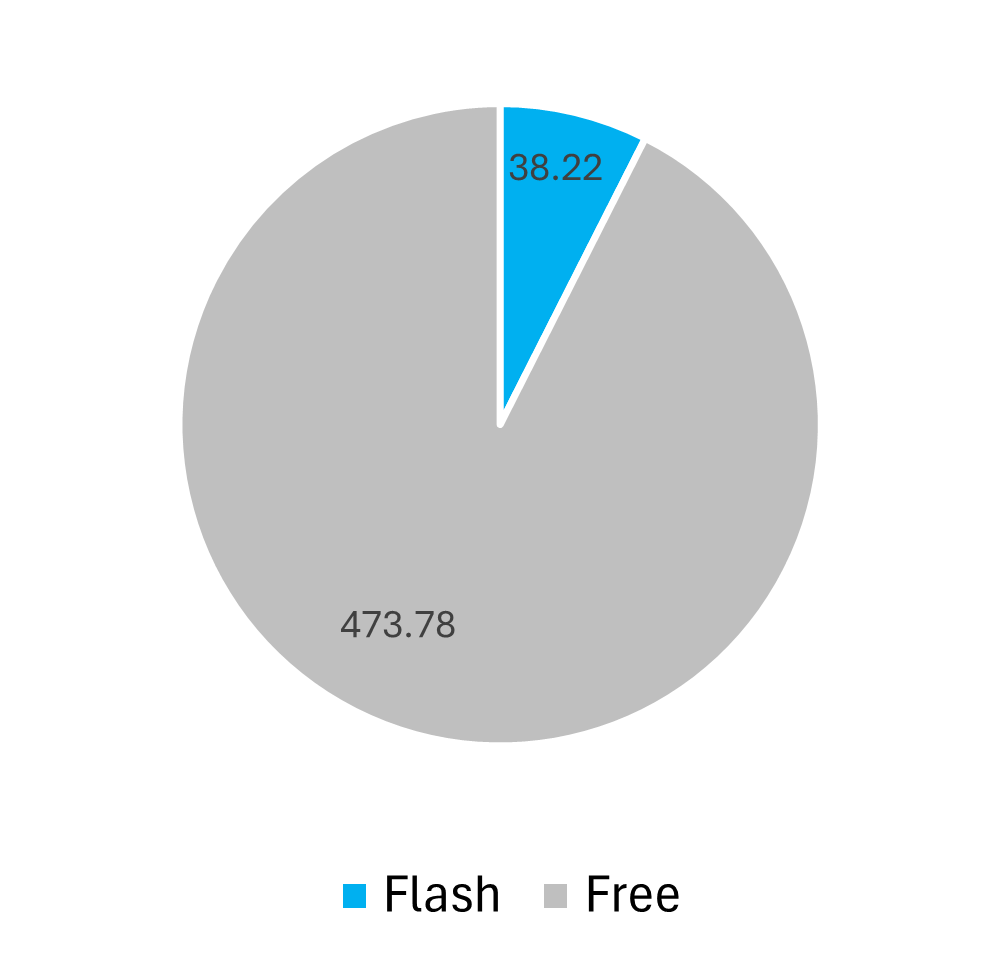
\includegraphics[width=\textwidth]{images/stm32flash.png}
         \caption{Dung lượng Flash}
\end{subfigure}
\hfill
\begin{subfigure}[b]{0.495\textwidth}
         \centering
         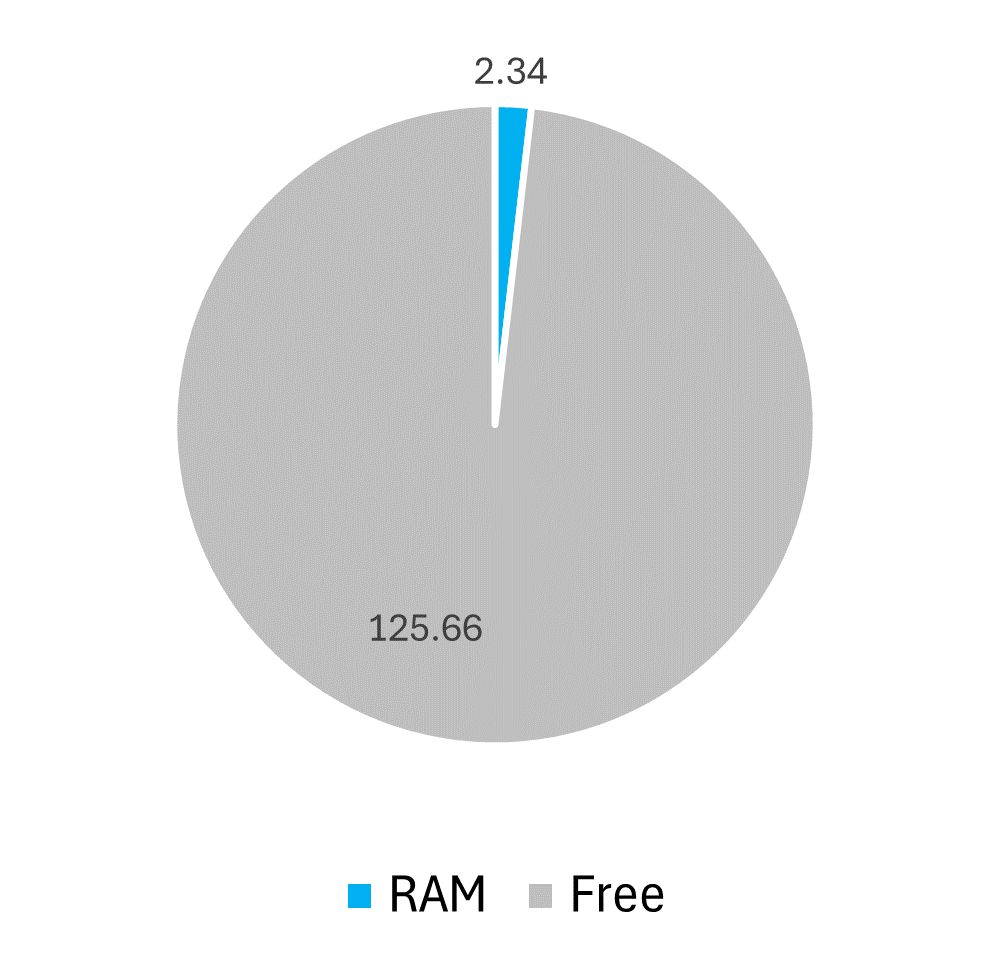
\includegraphics[width=\textwidth]{images/stm32ram.png}
         \caption{Dung lượng RAM}
\end{subfigure}
\caption{Dung lượng tiêu thụ của STM32F411VET6}
\label{fig:stm32mem}
\end{figure}

\begin{figure}[H]
\centering
\begin{subfigure}[b]{0.495\textwidth} 
         \centering
         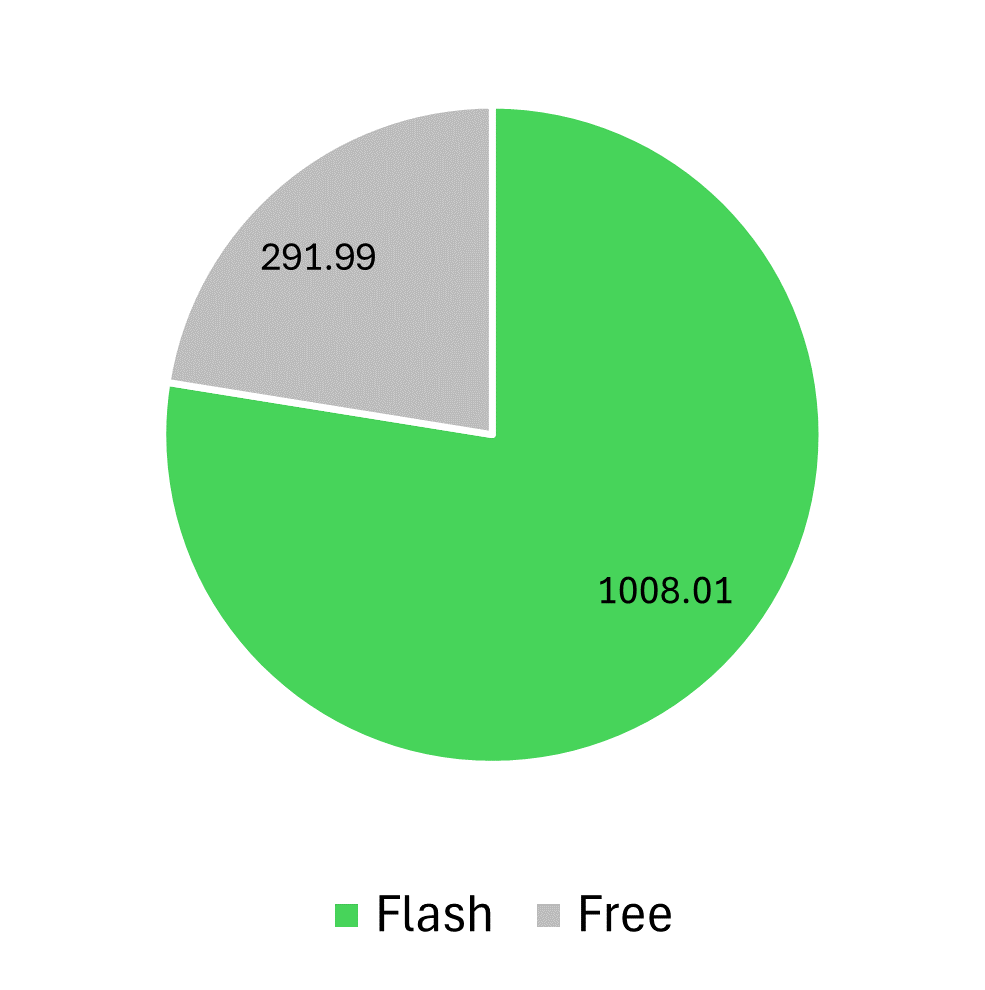
\includegraphics[width=\textwidth]{images/esp32flash.png}
         \caption{Dung lượng Flash}
\end{subfigure}
\hfill
\begin{subfigure}[b]{0.495\textwidth}
         \centering
         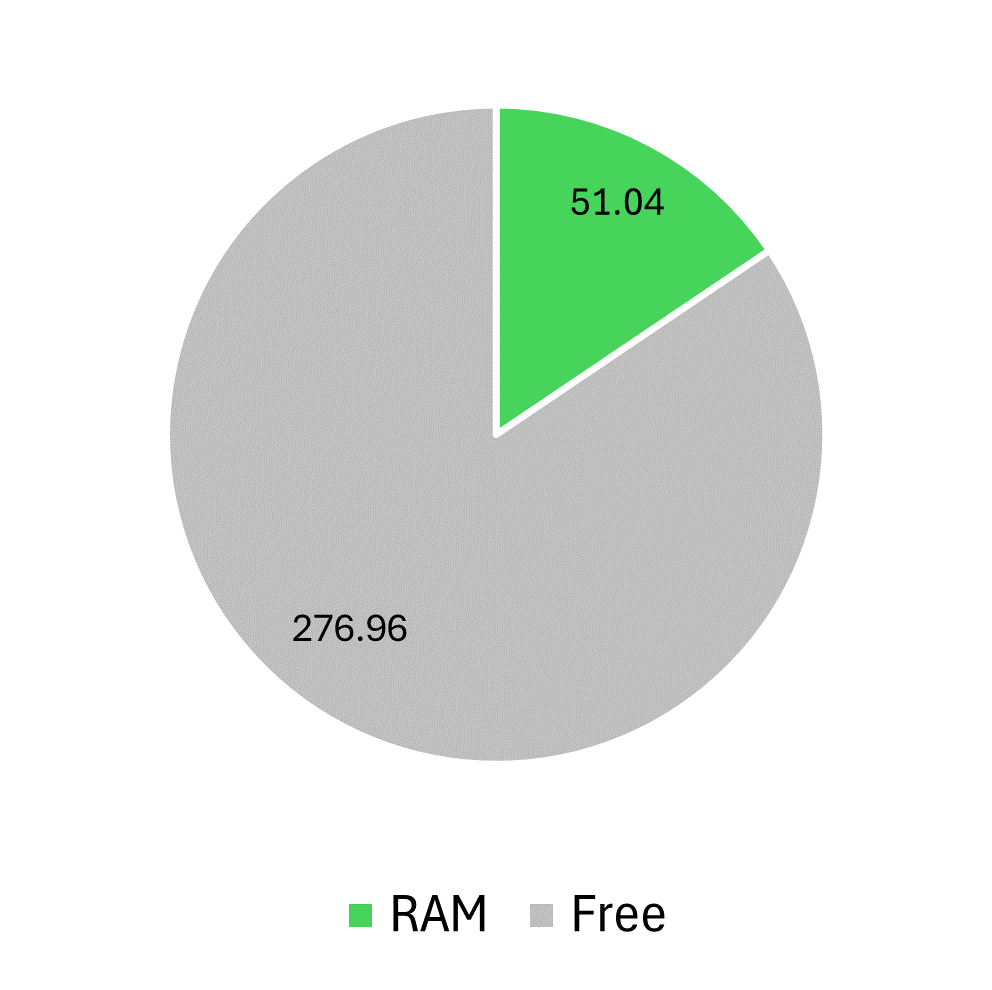
\includegraphics[width=\textwidth]{images/esp32ram.png}
         \caption{Dung lượng RAM}
\end{subfigure}
\caption{Dung lượng tiêu thụ của ESP32-WROOM-32}
\label{fig:esp32mem}
\end{figure}

\subsection{Phân tích công suất tiêu thụ}
Quá trình đo công suất tiêu thụ được thực hiện trên hệ thống phần cứng bao gồm vi điều khiển STM32F411VET6 ở lớp nhận thức và module ESP32 ở lớp mạng.
Cảm biến INA219 được sử dụng để phục vụ quá trình đo đạc của hệ thống. Đây là một cảm biến chuyên dụng sử dụng giao thức I2C cho phép
đo dòng điện, điện áp và tính toán công suất tiêu thụ với độ chính xác cao. Cả hệ thống được cấp nguồn chung là 5V và đo liên tục trong 60 phút. Quá trình trao đổi khóa cũng được cập nhật lại là trao đổi khóa sau mỗi 10 gói tin thành công.
Với cấu hình thử nghiệm như vậy sẽ cho ra cái nhìn khách quan hơn về mức tiêu thụ năng lượng của hệ thống.
Trong suốt quá trình đo, các thông như về dòng điện (mA) và công suất tiêu thụ (mW) được ghi lại mỗi phút. 
Các kết quả thu được phản ánh trực tiếp mức độ tiêu thụ năng lượng của từng thành phần cũng như toàn hệ thống trong suốt thời gian hoạt động.
\begin{figure}[H]
    \centering
    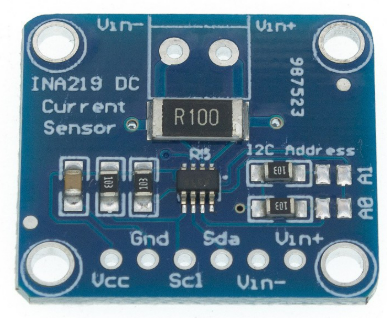
\includegraphics[width=0.2\linewidth]{ina219.png}
    \caption{Cảm biến dòng INA219}
    \label{fig:ina219}
\end{figure}

Hình \ref{fig:stm32pow} minh họa dòng điện và công suất tiêu thụ của STM32 trong suốt 60 phút. Dòng điện dao động trong khoảng từ 40 đến 48 mA, với giá trị trung bình đạt 43.99 mA. Công suất tiêu thụ của STM32 dao động từ 200 đến 240 mW, với mức trung bình trong một giờ là 222.97 mW.
\begin{figure}[H]
    \centering
    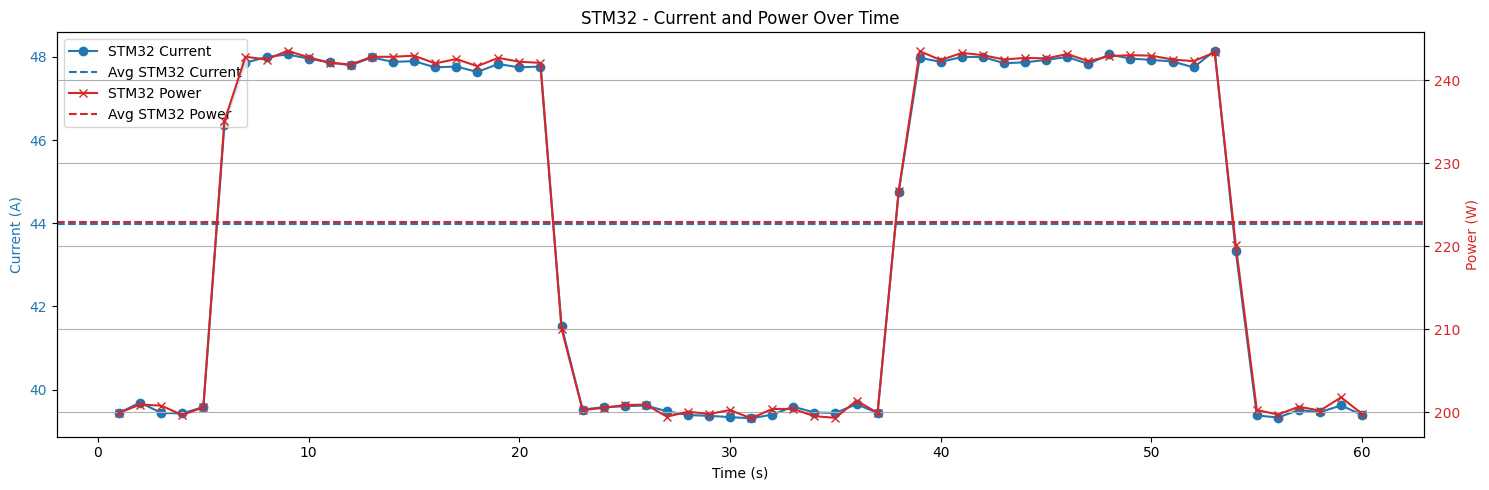
\includegraphics[width=1\linewidth]{stm32pow2.png}
    \caption{Mức tiêu thụ năng lượng của STM32F411VET6}
    \label{fig:stm32pow}
\end{figure}

Tương tự, hình \ref{fig:esp32pow} thể hiện đặc tính tiêu thụ năng lượng của ESP32 IoT Gateway. ESP32 có dòng điện dao động từ 100 đến 125 mA, với giá trị trung bình là 112.52 mA. 
Công suất tiêu thụ tương ứng dao động trong khoảng 500 đến 600 mW, với giá trị trung bình đạt 556.46 mW. 
Có thể nhận thấy ESP32 tiêu thụ năng lượng cao hơn đáng kể so với STM32, do phải xử lý các thuật toán phức tạp hơn, duy trì kết nối Wi-Fi và truyền dữ liệu liên tục tới máy chủ qua giao thức MQTT.

\begin{figure}[H]
    \centering
    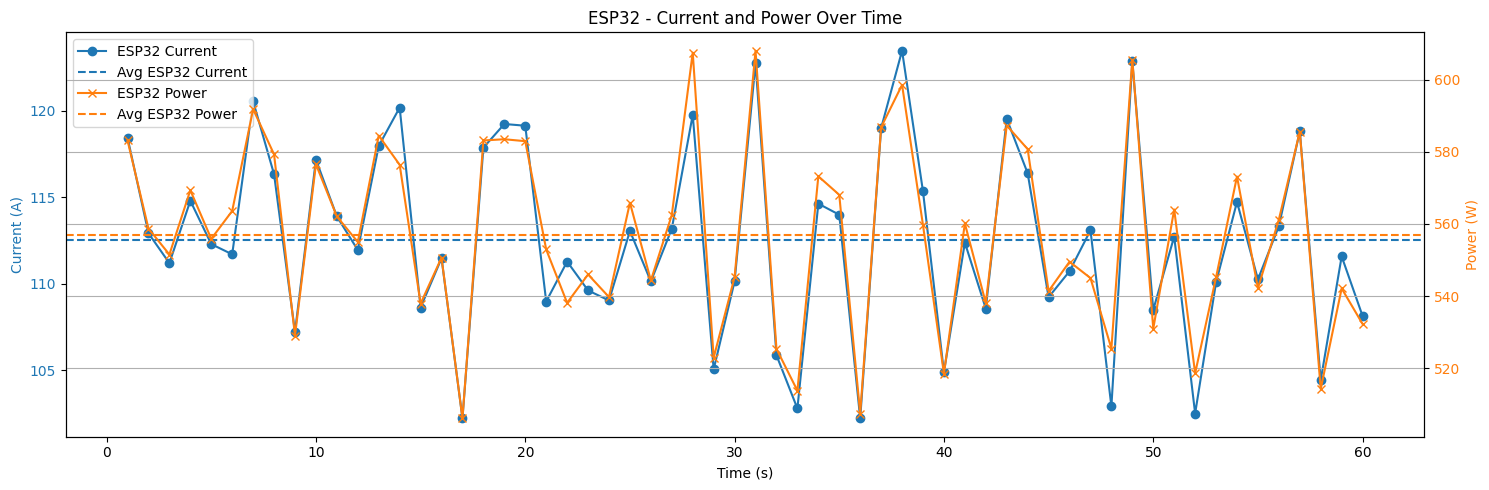
\includegraphics[width=1\linewidth]{esp32pow2.png}
    \caption{Mức tiêu thụ năng lượng của ESP32 Gateway}
    \label{fig:esp32pow}
\end{figure}


Hình \ref{fig:totalpow} trình bày mức tiêu thụ năng lượng tổng thể của toàn bộ hệ thống trong quá trình hoạt động. Kết quả cho thấy mức tiêu thụ trung bình đạt 779.43 mW.
Dựa trên kết quả này và đối chiếu với Bảng \ref{tab:hardware}, có thể phân loại hệ thống vào nhóm thiết bị IoT từ Category 1 đến Category 2, theo phân loại phần cứng được đề xuất bởi Abdulghani et al \cite{hardware}.
Điều này cho thấy kiến trúc hệ thống được thiết kế tối ưu, cân bằng tốt giữa hiệu quả năng lượng và khả năng bảo mật, qua đó tăng tính khả thi cho các ứng dụng thực tế, đặc biệt là trong các môi trường IoT có tài nguyên hạn chế.
\begin{figure}[H]
    \centering
    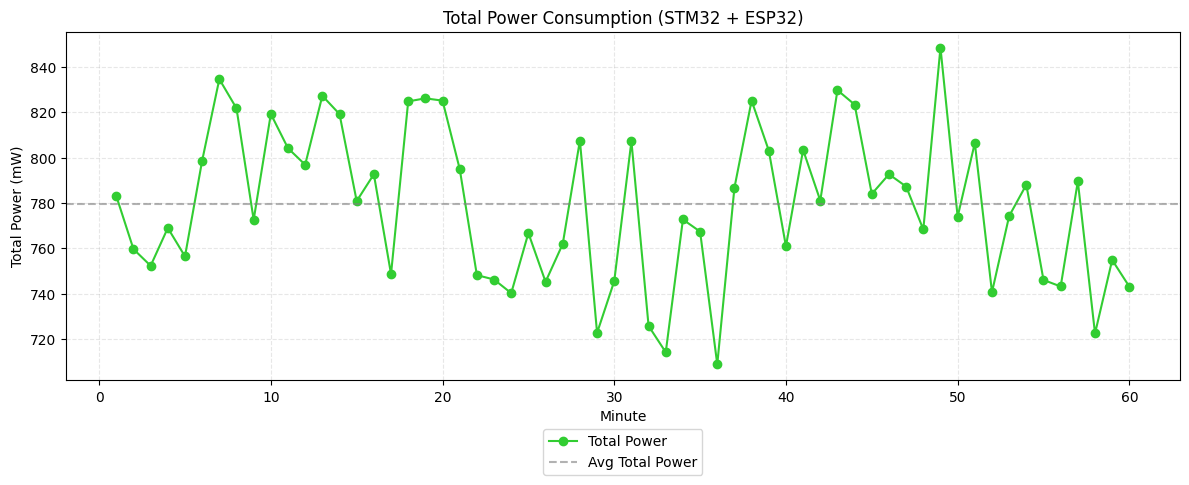
\includegraphics[width=0.9\linewidth]{totalpow.png}
    \caption{Mức tiêu thụ năng lượng của toàn bộ hệ thống}
    \label{fig:totalpow}
\end{figure}

\begin{table}[ht]
\centering
\small
\caption{Phân loại các thiết bị IoT dựa trên hiệu suất phần cứng}
\label{tab:hardware}
\begin{tabular}{|c|c|c|c|c|c|}
\hline
\textbf{Category} & \textbf{CPU} & \textbf{RAM} & \textbf{Storage} & \textbf{Power} & \textbf{Example} \\
\hline
Category~1 & 8-bit, 16~MHz & $\leq$~32~KB & Small & $\leq$~1~W & Arduino Mega \\
\hline
Category~2 & 32-bit, 80~MHz & 32--80~KB & Small & $\leq$~1~W & NodeMCU ESP-12 \\
\hline
Category~3 & Single-core, 1~GHz & 80~KB--512~MB & $\leq$~4~GB & 1--2~W & Raspberry Pi Zero \\
\hline
Category~4 & Quad-core, 1.2~GHz & 512~MB--2~GB & $\leq$~8~GB & 2--4~W & Raspberry Pi 3 \\
\hline
Category~5 & Quad-core, 2~GHz & $\geq$~8~GB & $\geq$~32~GB & High & Jetson TX2 \\
\hline
\end{tabular}
\begin{flushleft}
\footnotesize
Nguồn: Abdulghani, H.A.; Collen, A.; Nijdam, N.A. \textit{Guidance Framework for Developing IoT-Enabled Systems’ Cybersecurity}. Sensors 2023, 23, 4174. \url{https://doi.org/10.3390/s23084174}
\end{flushleft}
\end{table}

\subsection{Phân tích thông lượng và hiệu suất tải dữ liệu}
\label{sec:put}
Thông lượng và hiệu suất tải dữ liệu là hai thông số quan trọng trong việc đánh giá hệ thống. Việc sử dụng kiến trúc khung truyền với các trường dữ liệu bổ sung sẽ tốn thêm chi phí truyền tải, kích thước mỗi gói tin sẽ tăng so với các phương pháp đơn giản hơn. Phần này sẽ tập trung vào phân tích thông lượng và hiệu suất tải dữ liệu để đánh giá một số hạn chế của hệ thống. Đồng thời, đề xuất một số phương pháp có thể giúp cải thiện hệ thống trong tương lai.

Khung truyền GS2 sẽ được sử dụng trong việc đánh giá thông lượng cũng như hiệu suất tải dữ liệu của hệ thống. Đây là khung truyền được sử dụng với tần suất lớn nhất trong suốt quá trình truyền tải dữ liệu. Khung truyền GS2 là khung truyền đảm nhận việc truyền dữ liệu từ lớp nhận thức đến máy chủ bằng giao thức MQTT. Thông qua việc phân tích khung truyền GS2, có thể xấp xỉ chính xác nhất thông lượng và hiệu suất tải dữ liệu của hệ thống. Tổng kích thước của khung truyền GS2 là tổng kích thước của tất cả các trường dữ liệu được tính toán như sau:
\begin{align*}
\text{Size}_{GS2} &= \text{SOF (2)} + \text{ID (4)} + \text{Packet Type (1)} + \text{Seq. Number (4)} \\
& \quad + \text{Nonce (16)} + \text{Payload Length (1)} + \text{Encrypted Payload (3)} \\
& \quad + \text{Auth Tag (16)} + \text{EOF (2)} \\
&= 49\ \text{bytes}
\end{align*}
Trong hệ thống đã triển khai, lớp nhận thức thu thập và truyền tải 3 byte dữ liệu, từ đó tham số \textit{Encrypted Payload} cũng có kích thước là 3 byte. Một điều chú ý đó là tổng kích thước của khung truyền GS2 sẽ có sự thay đổi dựa trên kích thước dữ liệu mà lớp nhận thức muốn truyền tải. Từ kết quả đó được ở phần \ref{sec:res}, trong 120 phút, hệ thống đã truyền tải tổng cộng 147,682 gói tin. Tuy nhiên, vì phần này chỉ đánh giá thông lượng của khung truyền GS2, 120 khung truyền GS1 trong việc trao đổi khóa sẽ bị loại bỏ trong tính toán. Dẫn đến tổng số gói tin sử dụng khung truyền GS2 sẽ được tính là:
\[
\text{Total}_{GS2} = 147,682 - 120 = 147,562 \ \text{(gói tin)}
\]
Tổng kích thước mà hệ thống đã truyền tải sẽ được tính như sau:
\[
\text{Total}_{size} = 147,562 \times 49 = 7,230,538 \ \text{(byte)}
\]
Từ đó, ta có thể tính toán thông lượng của hệ thống bằng công thức:
\[
\textit{Throughtput} = \left( \frac{\text{Data size}}{\text{Transmission Time}} \right) \times 8 = \left( \frac{7,230,538}{120 \times 60} \right) \times 8 \approx 8,033.93 \ \text{bps}
\]
Trong đánh giá này, mỗi khung truyền GS2 có tổng kích thước là 49 byte, tuy nhiên chỉ có 3 byte dữ liệu cần thiết, phần còn lại chủ yếu là các trường bổ sung nhằm đảm bảo tính bảo mật của hệ thống, dẫn đến một tham số được đưa ra đó là hiệu suất tải (\textit{payload efficiency}) khá nhỏ là $3/49 \approx 6.12\%$. Con số này nói lên rằng chỉ có 6.12\% dữ liệu được truyền là dữ liệu hữu ích, trong khi phần còn lại là chi phí truyền dẫn khác không có ý nghĩa đối với người dùng cuối. Vì vậy, mặc dù thông lượng của hệ thống khá cao nhưng thực tế thì thông lượng hữu ích (goodput) lại thấp hơn nhiều:
\[
\textit{Goodput} = \left( \frac{147,562 \times 3}{120 \times 60} \right) \times 8 \approx 491.87 \ \text{bps}
\]
Từ những phân tích trên, có thế thấy chi phí truyền tải khi áp dụng kiến trúc khung truyền là không nhỏ. Với hiệu suất tải thấp sẽ dẫn đến việc tiêu tốn băng thông, băng thông sẽ không được sử dụng một cách tối ưu. Tuy nhiên, hiệu suất tải sẽ được cải thiện đáng kể nếu hệ thống truyền nhiều dữ liệu, tức là kích thước tải lớn hơn. Bảng \ref{tab:efficiency} và hình \ref{fig:charteff} trình bày hiệu suất tải với các kích thước tải khác nhau trên cũng một khung truyền dữ liệu. Có thể thấy thay vì truyền 3 byte dữ liệu như đề tài đã thực hiện, nếu ứng dụng kiến trúc này vào các hệ thống cần truyền nhiều dữ liệu đồng thời, việc sử dụng băng thông sẽ được tối ưu hơn rất nhiều.
Biểu đồ ở hình \ref{fig:charteff} cho thấy xu hướng với kích thước tải càng lớn, hiệu suất tải càng cải thiện.
\begin{table}[h]
\centering
\small
\caption{Hiệu suất tải với các kích thước tải khác nhau}
\label{tab:efficiency}
\begin{tabular}{|p{4cm}|p{5cm}|p{3cm}|}
\hline
Payload Length & Total Frame Size & Efficiency \\
\hline
3 bytes   & 49 bytes  & 6.12\%  \\
10 bytes  & 56 bytes & 17.85\% \\
20 bytes  & 66 bytes & 30.30\% \\
50 bytes  & 96 bytes & 52.08\% \\
\hline
\end{tabular}
\end{table}

\begin{figure}[H]
    \centering
    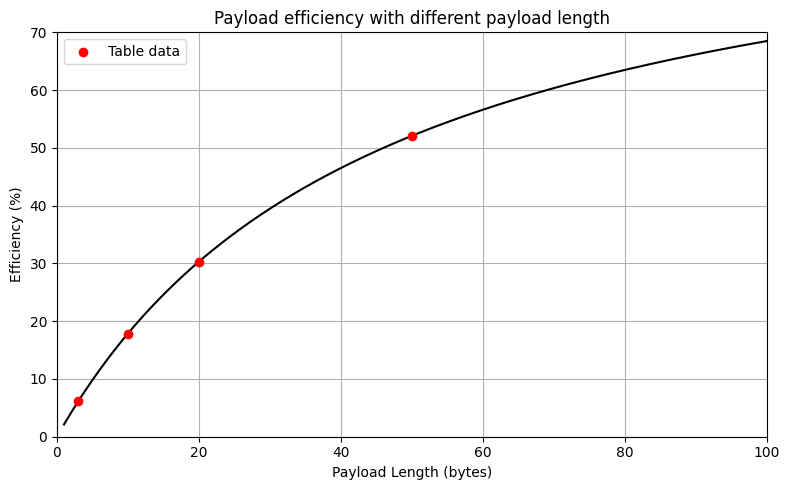
\includegraphics[width=0.75\linewidth]{chartefficiency.png}
    \caption{Hiệu suất tải với các kích thước tải khác nhau}
    \label{fig:charteff}
\end{figure}

\subsection{Phân tích khả năng bảo mật của hệ thống}
Phần này trình bày đánh giá chi tiết về mức độ an toàn của hệ thống IoT được đề xuất, thông qua việc phân tích và nhận xét khả năng kháng cự của nó trước một số dạng tấn công phổ biến hiện nay.

\textit{Nhận xét 1: Hệ thống có khả năng chống lại các cuộc tấn công từ bên ngoài như Man-in-the-Middle}
\begin{itemize}
    \item Trong kiến trúc đề xuất, tất cả các lớp trong mô hình IoT bốn lớp đều được mã hóa bằng thuật toán mã hóa xác thực Ascon-128a. Nhờ đó, dù kẻ tấn công có xâm nhập và đánh cắp dữ liệu tại bất kỳ lớp nào trong quá trình truyền giữa, dữ liệu vẫn không thể bị giải mã hay sử dụng trái phép. Cơ chế này giúp đảm bảo tính bảo mật và toàn vẹn của thông tin người dùng trong toàn bộ hệ thống.
\end{itemize}

\textit{Nhận xét 2: Cơ chế khung truyền được thiết kế để ngăn chặn các thiết bị không hợp lệ giao tiếp với hệ thống.}
\begin{itemize}
    \item Với thiết kế khung truyền dữ liệu, đảm bảo rằng chỉ có những thiết bị cùng một hệ sinh thái mới có thể giao tiếp và truyền dữ liệu cho nhau. Các thiết bị khác ở bên ngoài sẽ không có khả năng gửi dữ liệu vì không khớp ở các trường như SOF, Identifier ID và EOF, đây vốn là những trường độc nhất được cấu hình riêng cho mỗi thiết bị.
\end{itemize}

\textit{Nhận xét 3: Cơ chế khung truyền đảm bảo tính toàn vẹn của dữ liệu.}
\begin{itemize}
    \item Trước khi truyền, dữ liệu luôn được cấu trúc lại thành khung truyền bao gồm các trường xác thực. Khi một lớp trong hệ thống tiếp nhận khung truyền, dữ liệu sẽ được kiểm tra thông qua hàm phân giải nhằm xác thực tính hợp lệ. Cơ chế này giúp phát hiện và loại bỏ các sai sót trong quá trình truyền, đảm bảo rằng dữ liệu đến đích luôn chính xác. Điều này được thể hiện thông qua chỉ số PDR đạt 99.99\% trong quá trình thử nghiệm.
\end{itemize}

\textit{Nhận xét 4: Quá trình trao đổi khóa được đảm bảo an toàn nhờ tích hợp thẻ xác thực (Auth Tag) trong khung truyền.}
\begin{itemize}
    \item Để bảo vệ quá trình trao đổi khóa, khóa công khai được truyền với khung truyền được tích hợp 16 byte Auth Tag. Với sự kết hợp của Auth Tag, đảm bảo rằng kể cả khi có kẻ tấn công từ bên ngoài muốn gửi khóa công khai giả nhằm phá hoại việc tính toán khóa bí mật, hệ thống vẫn có thể phát hiện và từ chối các khóa giả ngay lập tức. 
\end{itemize}

\textit{Nhận xét 5: Thuật toán trao đổi khóa ECDH đảm bảo mức độ bảo mật theo khuyến nghị của NIST.}
\begin{itemize}
    \item Quá trình trao đổi khóa dùng thuật toán ECDH sử dụng đường cong \textit{sect163k1} với mức bảo mật là 80-bit. Mức bảo mật này đáp ứng được khuyến nghị của NIST về mức độ bảo mật \cite{nist}. Hơn nữa, khóa bảo mật sẽ được cập nhật định kỳ, khiến các cuộc tấn brute-force vào khóa bí mật trở nên bất khả thi.
\end{itemize}

\textit{Nhận xét 6: Hệ thống có khả năng phát hiện và ngăn chặn các cuộc tấn công phát lại (replay attack).}
\begin{itemize}
    \item Với 4 byte \textit{sequence number} được tích hợp trong khung truyền GS2, đảm bảo rằng máy chủ có thể phát hiện và từ chối bất kỳ gói tin nào bị gửi lại do không trùng khớp \textit{sequence number}. Nhờ đó, các cuộc tấn công phát lại sẽ không thể làm gián đoạn hệ thống.
\end{itemize}

\textit{Nhận xét 7: Cơ chế safe counter giúp chống lại tấn công brute-force vào sequence number của hệ thống.}
\begin{itemize}
    \item Một kịch bản có thể xảy ra đó là kẻ tấn công cố gắng brute-force toàn bộ 4 byte \textit{sequence number} để có thể thành công gửi gói tin vào máy chủ. Vì vậy, cơ chế \textit{safe counter} được thiết lập để có thể các cuộc tấn công trên. Nếu máy chủ từ chối một số lượng gói tin nhất định, gateway và máy chủ sẽ sử dụng \textit{safe counter} để cập nhật lại \textit{sequence number} mới một cách đồng bộ. Với cơ chế này, tỉ lệ brute-force thành công gần như là không thể xảy ra. 
\end{itemize}

\textit{Nhận xét 8: Khả năng chống lại tấn công kênh biên (side-channel attack) nhờ vào mã hóa Ascon.}
\begin{itemize}
    \item Khả năng chống lại tấn công kênh biên được chứng minh trong bài báo \cite{asconv1.2} của nhóm nghiên cứu Ascon. Trong đó họ đã đề cập đến việc
    Ascon có thể được triển khai hiệu quả trên các nền tảng và ứng dụng yêu cầu khả năng chống tấn công kênh bên cao. Việc sử dụng S-box theo dạng bitsliced giúp ngăn chặn các cuộc tấn công dựa trên thời gian truy cập bộ nhớ cache, vì không cần sử dụng bảng tra cứu (lookup table). Ngoài ra, bậc đại số thấp của S-box còn tạo điều kiện thuận lợi cho việc áp dụng các biện pháp bảo vệ kênh bên ở cả cấp độ thứ nhất và cao hơn, thông qua các kỹ thuật như masking (che giấu dữ liệu) hoặc chia sẻ (sharing-based countermeasures). 
\end{itemize}

\textit{Nhận xét 9: Hệ thống đã được kiểm nghiệm thực tế với lượng lớn dữ liệu giả mạo và cho thấy khả năng phòng thủ cao.}
\begin{itemize}
    \item Hệ thống đã được kiểm tra bằng cách gửi 70,000 gói tin giả mạo. Rõ ràng rằng nếu kẻ tấn công không biết được kiến trúc của khung truyền dữ liệu, họ sẽ không thể gửi dữ liệu tới hệ thống. Vì vậy, trong thử nghiệm, giả định kẻ tấn công biết trước khung truyền dữ liệu cho từng giao tiếp. Kết quả vẫn cho thấy máy chủ đã từ chối toàn bộ 70,000 gói tin giả mạo, đạt tỉ lệ 100\%, chứng minh khả năng bảo vệ của hệ thống trước các cuộc tấn công trên.
\end{itemize}

\textit{Nhận xét 10: Kiến trúc đề xuất triển khai phù hợp với các thiết bị IoT.}
\begin{itemize}
    \item Đề tài sử dụng các phần cứng tầm trung như STM32F411VET6 và ESP32, xung nhịp của STM32 cũng được giới hạn ở mức mặc định là 16MHz. Tuy nhiên, với các phân tích về sử dụng bộ nhớ, thời gian xử lý dữ liệu cũng như mức năng lượng tiêu thụ ở phần \ref{sec:res}, có thể thấy kiến trúc IoT đề tài đề xuất hoàn toàn phù hợp để triển khai trên các thiết bị IoT có khả năng tính toán thấp mà vẫn cung cấp tính năng bảo mật tốt. Các dòng vi điều khiển cao cấp hơn như STM32F7 hoặc STM32H7, kết hợp với Raspberry Pi như một IoT Gateway thì hiệu suất thậm chí sẽ vượt trội hơn nhưng các phần cứng tầm trung là hoàn toàn đủ để triển khai tốt kiến trúc này.
\end{itemize}


% \begin{enumerate}
%     \item Với thiết kế khung truyền dữ liệu, đảm bảo rằng chỉ có những thiết bị cùng một hệ sinh thái mới có thể giao tiếp và truyền dữ liệu cho nhau. Các thiết bị khác ở bên ngoài sẽ không có khả năng gửi dữ liệu vì không khớp ở các trường như SOF, Identifier ID và EOF, đây vốn là những trường độc nhất được cấu hình riêng cho mỗi thiết bị.
%     \item Để bảo vệ quá trình trao đổi khóa, khóa công khai được truyền với khung truyền được tích hợp 16 byte Auth Tag. Với sự kết hợp của Auth Tag, đảm bảo rằng kể cả khi có kẻ tấn công từ bên ngoài muốn gửi khóa công khai giả nhằm phá hoại việc tính toán khóa bí mật, hệ thống vẫn có thể phát hiện và từ chối các khóa giả ngay lập tức.   
%     \item Quá trình trao đổi khóa dùng thuật toán ECDH sử dụng đường cong \textit{sect163k1} với mức bảo mật là 80-bit. Mức bảo mật này đáp ứng được khuyến nghị của NIST về mức độ bảo mật \cite{?}. Hơn nữa, khóa bảo mật sẽ được cập nhật định kỳ, khiến các cuộc tấn brute-force vào khóa bí mật trở nên không khả thi.
%     \item Với 4 byte \textit{sequence number} được tích hợp trong khung truyền GS2, đảm bảo rằng máy chủ có thể phát hiện và từ chối bất kỳ gói tin nào bị gửi lại do không trùng khớp \textit{sequence number}. Nhờ đó, các cuộc tấn công phát lại sẽ không thể làm gián đoạn hệ thống.
%     \item Một kịch bản có thể xảy ra đó là kẻ tấn công cố gắng brute-force toàn bộ 4 byte \textit{sequence number} để có thể thành công gửi gói tin vào máy chủ. Vì vậy, cơ chế \textit{safe counter} được thiết lập để có thể các cuộc tấn công trên. Nếu máy chủ từ chối một số lượng gói tin nhất định, cả gateway và máy chủ sẽ sử dụng \textit{safe counter} để cập nhật lại \textit{sequence number} mới. Với cơ chế này, tỉ lệ brute-force thành công gần như là không thể. 
%     \item Hệ thống đã được kiểm tra bằng cách gửi 70,000 gói tin giả mạo. Rõ ràng rằng nếu kẻ tấn công không biết được kiến trúc của khung truyền dữ liệu, họ sẽ không thể gửi dữ liệu tới hệ thống. Vì vậy, trong thử nghiệm, giả định rằng kẻ tấn công biết trước khung truyền dữ liệu cho từng giao tiếp. Kết quả vẫn cho thấy máy chủ đã từ chối toàn bộ 70,000 gói tin giả mạo, đạt tỉ lệ 100\%, chứng minh khả năng bảo vệ của hệ thống trước các cuộc tấn công trên.
% \end{enumerate}
